\documentclass[18pt]{beamer}
\usepackage[utf8]{inputenc} % for the umlauts
\usepackage{subcaption}

\beamertemplatenavigationsymbolsempty
%% SLIDE FORMAT

% use 'beamerthemekit' for standard 4:3 ratio
% for widescreen slides (16:9), use 'beamerthemekitwide'

\usepackage{templates/beamerthemekit}
\usepackage{stackengine}
\usepackage{graphicx}
\usepackage{verbatim}
\usepackage{tikz}
\usepackage{tikz-uml}
\usepackage{caption}
\captionsetup[figure]{labelformat=empty}% redefines the caption setup of the figures environment in the beamer class.

% \usepackage{templates/beamerthemekitwide}

\setcounter{tocdepth}{1}

%% TITLE PICTURE

% if a custom picture is to be used on the title page, copy it into the 'logos'
% directory, in the line below, replace 'mypicture' with the 
% filename (without extension) and uncomment the following line
% (picture proportions: 63 : 20 for standard, 169 : 40 for wide
% *.eps format if you use latex+dvips+ps2pdf, 
% *.jpg/*.png/*.pdf if you use pdflatex)

%\titleimage{mypicture}

%% TikZ INTEGRATION

% use these packages for PCM symbols and UML classes
 \usepackage{templates/tikzkit}
	\usepackage{templates/tikzuml}

% the presentation starts here

\usepackage[absolute,overlay]{textpos}
\usepackage{csquotes}
%\usepackage[texcoord,grid,gridunit=mm,gridcolor=red, subgridcolor=green]{eso-pic}
\setbeamercovered{invisible}

\title[SWT1]{Softwaretechnik 1 - 1. Tutorium}
\subtitle{Tutorium 17}
\author{Felix Bachmann}
\date{14.05.2019}

\institute{KIT - Institut für Programmstrukturen und Datenorganisation (IPD)}

% Bibliography


\begin{document}

% change the following line to "ngerman" for German style date and logos
\selectlanguage{ngerman}

%title page
\begin{frame}
\titlepage
\end{frame}

%table of contents
\begin{frame}{Themenübersicht}
\tableofcontents
\end{frame}

\section{Orga}

	\begin{frame}{Ersatztermin}

	\centering
	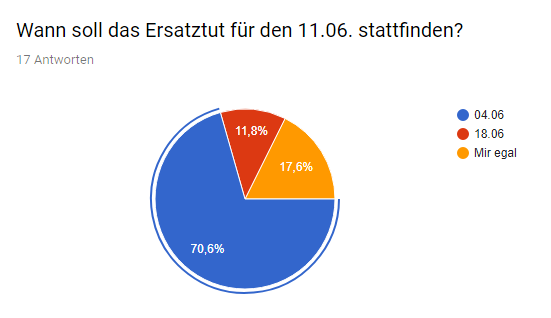
\includegraphics[scale=0.7]{pics/tut1/poll.png}
		\begin{itemize}
		\item Tut von 11.06 wird auf 04.06. verschoben
		\item ansonsten alles gleich (11:30-13:00, -119) 
	\end{itemize}
\end{frame}


	\subsection{Feedback 1. Übungsblatt}
	\begin{frame}
		\frametitle{1. Übungsblatt Statistik}
		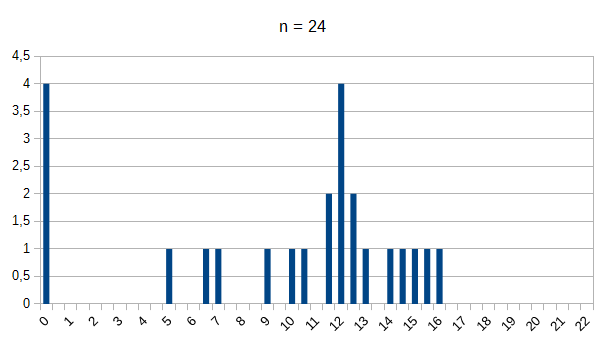
\includegraphics[scale=0.7]{./pics/tut1/statistics_ub1.png}
	\end{frame}
	
	\subsection{1. Übungsblatt - Fehler (Allgemein)}
	\begin{frame}
		\frametitle{Allgemeine Anmerkungen}
			\begin{itemize}
			\item für Feedback zu eurem Code Deckblatt einwerfen!
		\end{itemize}
		\begin{block}{Punktevergabe}
			generell ohne Abzug
			\begin{itemize}
				\item gleiche Abgabe bei allen Aufgaben
			\end{itemize}
			\pause
			generell mit Abzug
			\begin{itemize}
				\item Code nicht CheckStyle-konform (auch Tests!) 
				\begin{itemize}
					\item Save Actions bei Eclipse! (IntelliJ ähnlich)
				\end{itemize}
				\item JavaDoc nicht (vollständig \&\& sinnvoll)
				\item Git-Commits nicht (regelmäßig \&\& aussagekräftig)
			\end{itemize}
		\end{block}
	\end{frame}

\begin{frame}
\frametitle{Allgemeine Anmerkungen - pom.xml}

\begin{block}{Abhängigkeiten deklarieren}
\begin{itemize}
		\item iMage dient dazu jmjrst.main zu verpacken
		\item wenn ihr Abhängigkeiten in iMage-pom hinzufügt funktioniert es bei euch
		\begin{itemize}
			\item aber es wird jmjrst.main-pom in zip gepackt
			\item bei mir explodiert es, da mein iMage die Abhängigkeit nicht hat
		\end{itemize}
	\end{itemize}
 Lösung: Abhängigkeiten in dem Untermodul, das ihr gerade abgebt, deklarieren
\end{block}
\pause
\begin{block}{Parent}
	\begin{itemize}
		\item als parent von Untermodulen iMage, nicht das remote uebungsparent benutzen!
		\item als Version des Parents 0.0.1-SNAPSHOT
	\end{itemize}
\end{block}
\pause
ab nächstem ÜB Punktabzug, wenn ich noch irgendwas an der pom ändern muss, damit es bei mir läuft 
\end{frame}
	
	\subsection{1. Übungsblatt - Fehler (Aufgabe 1)}
	\begin{frame}
		\frametitle{Häufige Fehler}
		\begin{block}{Aufgabe 1 (Altsoftware vorbereiten)}
		\begin{itemize}
			\item falsche oder keine .gitignore in die zip verpackt 
			\begin{itemize}
				\item Konfiguration in src/assembly/src.xml
				\item wenn ihr nur .gitignore hinschreibt, wird .gitignore aus jmjrst-Ordner genommen
				\item die existiert bei euch vielleicht garnicht, oder ist default
				\begin{itemize}
					\item in zip liegt keine oder falsche .gitignore
				\end{itemize}
				\item fix: ../../.gitignore statt .gitignore
			\end{itemize}
			\pause
			\item LICENSE sollte in das Wurzelverzeichnis
			\begin{itemize}
				\item siehe \url{https://maven.apache.org/guides/introduction/introduction-to-the-standard-directory-layout.html}
			\end{itemize}
		\end{itemize}
		\end{block}
	\end{frame}
	
	\subsection{1. Übungsblatt - Fehler (Aufgabe 2)}
	\begin{frame}
		\frametitle{Häufige Fehler}
		\begin{block}{Aufgabe 2 + 3 (Modultests + Testüberdeckung)}
			\begin{itemize}
				\item CheckStyle (und JavaDoc) auch in Tests benutzen \pause
				\item sinnvolle Definition der Gleichheit zweier Bilder
				\begin{itemize}
					\item gleiche Dimensionen
					\item UND gleiche Pixel-Werte
				\end{itemize} \pause
				\item auch bei Drehung um 0$^{\circ}$  ist Überprüfung von Gleichheit nötig \pause
				\item \texttt{assertEquals()} reicht nicht aus, um Gleichheit der Bilder zu prüfen \pause 
				\item Ordner \texttt{target/test} wurde nicht erstellt
				\begin{itemize}
					\item \texttt{new File()} erstellt keine Datei, sondern nur einen "'pointer"' auf einen Pfad (siehe \texttt{File.createNewFile()} oder \texttt{File.mkdir()} oder \texttt{File.mkdirs())} \pause
				\end{itemize}
				\item \texttt{@Test(expected=XYException.class)} nutzen, wenn Exception erwartet, sonst \texttt{@Ignore}
			\end{itemize}
		\end{block}
	\end{frame}
	
\begin{frame}
	\frametitle{Häufige Fehler}
	\begin{block}{Aufgabe 2 + 3 (Modultests + Testüberdeckung)}
		\begin{itemize}
			\item Stil: Konstanten für Pfade benutzen
			\begin{itemize}
				\item magic Strings sind ähnlich böse wie magic numbers
			\end{itemize}
			\pause
			\item Generator soll in \texttt{@Before}-Methode vor jedem Test neu erstellt werden
			\begin{itemize}
				\item Objekt soll \enquote{frisch} sein
				\item Zustand des Objektes kann sich durch Methoden-Aufrufe verändern
			\end{itemize}
			\pause
			\item niemals absolute Pfade verwenden
			\begin{itemize}
				\item ich habe bei mir keinen Ordner \texttt{C:/Users/Manfred/Desktop/Uni/bloedes\_SWT/eclipseWorkspace/\dots}
				\item besser: relative Pfade 
				\item am besten: Resourcen über eingebaute Methoden suchen
				\begin{itemize}
					\item \texttt{this.getClass().getResource(<Datei-Name>)}
					\item \dots
					\item siehe \url{https://stackoverflow.com/questions/3861989/preferred-way-of-loading-resources-in-java}
				\end{itemize}
			\end{itemize}
		\end{itemize}
	\end{block}
\end{frame}

\section{Wasserfallmodell}
	\subsection{Wasserfallmodell, ohne Grafik}
	\begin{frame}
		\frametitle{Wasserfallmodell}
		\begin{itemize}
			\item Was ist das? 
			\item Weiß jemand die Phasen? :)
		\end{itemize}
	\end{frame}
	
	\subsection{Wasserfallmodell, mit Grafik}
	\begin{frame}
		\frametitle{Wasserfallmodell}
		\begin{itemize}
			\item \textcolor{red}{dokumentengetriebenes Prozessmodell} \pause
			\item mögliche Phasen der Softwareentwicklung \pause
		\end{itemize}
		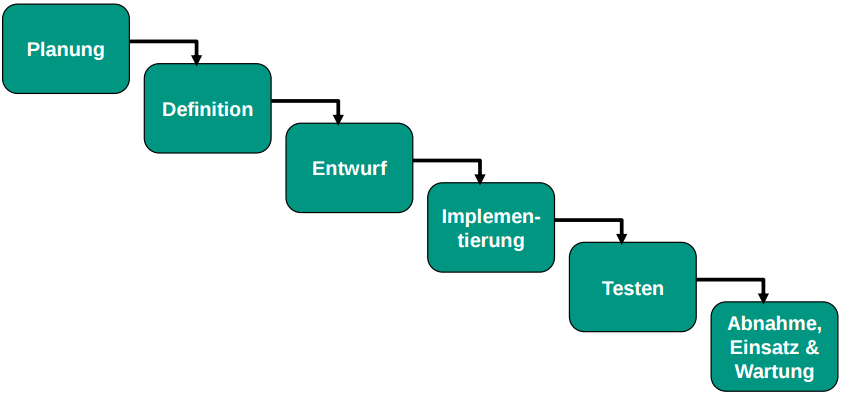
\includegraphics[scale=0.4]{./pics/tut1/waterfall_without-docs.png}
		\pause
		Probleme?
	\end{frame}
	
	\subsection{Wasserfallmodell, mit Grafik und Dokumenten}
	\begin{frame}
		\frametitle{Wasserfallmodell}
		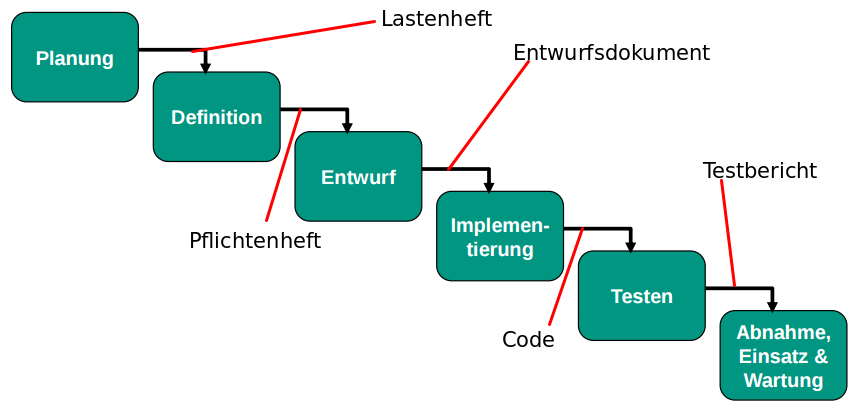
\includegraphics[scale=0.4]{./pics/tut1/waterfall_with-docs.png}
		\pause
		Dokumente für das 2. ÜB: 
		\begin{itemize}
			\item Lastenheft
			\item Durchführbarkeitsuntersuchung (weiteres Artefakt der Planung)
		\end{itemize}
	\end{frame}

\section{Durchführbarkeitsuntersuchung}
	\subsection{Welche Aspekte?}
	\begin{frame}
		\frametitle{Durchführbarkeitsuntersuchung}
		\begin{block}{Grundlegende Frage}
			Ist das Projekt in dem jeweiligen Szenario überhaupt durchführbar?
		\end{block}
		\begin{enumerate}
			\item \pause Fachlich \pause (softwaretechnisch leicht realisierbar?) \pause
			\item Alternativen \pause (lieber altes Projekt anpassen oder komplett neu entwickeln?) \pause
			\item Personell \pause (genug qualifizertes Personal?) \pause
			\item Risiken \pause (Gibt es Risiken? :D) \pause
			\item Ökonomisch \pause (wirtschaftlich? Termine?) \pause
			\item Rechtlich \pause (Datenschutz, Standards)
		\end{enumerate}
		\pause
		\begin{alertblock}{Fürs Übungsblatt}
			Denkt euch was (plausibles) aus!
		\end{alertblock}
	\end{frame}

\section{Lastenheft}
	\subsection{Lastenheft - Gliederung}
	\begin{frame}
		\frametitle{Lastenheft}
		\begin{block}{Grundlegende Aufgabe}
			Das Lastenheft sammelt die Anforderungen des Auftraggebers an den Auftragnehmer. Theoretisch vom Kunden geschrieben.
		\end{block}
		\begin{enumerate}
			\item \pause Zielbestimmung (grobe Beschreibung) \pause 
			\item Produkteinsatz (Für wen? Zielgruppe, Anwendungsbereich)\pause
			\item Funktionale Anforderungen (feingranular: Funktionen des Produkts)\pause 
			\item Produktdaten (Welche Daten speichern?)\pause
			\item Nichtfunktionale Anforderungen (Meta-Anforderungen: Zeit, Zuverlässigkeit)\pause 
			\item Systemmodelle
			\begin{itemize}
				\item Szenarien (spezielles Beispiel)
				\item Anwendungsfälle (allgemeiner Verwendungszweck)
			\end{itemize}
			\pause
			\item Glossar (technische Begriffe erklären)
		\end{enumerate}
	\end{frame}
	
	\subsection{Lastenheft - Unterschiede}
	\begin{frame}
		\frametitle{Begriffsklärung}
		\begin{block}{Zielbestimmung vs. Funktionale Anforderungen}
			\pause
			\begin{itemize}
				\item Zielbestimmung: allgemeine Beschreibung, was das Produkt können soll
				\item Funktionale Anforderungen: konkrete Auflistung von Funktionen
			\end{itemize}
		\end{block}
		\pause
		\begin{block}{Funktionale Anforderungen vs. Nichtfunktionale Anforderungen}
			\pause
			\begin{itemize}
				\item Funktionale Anforderungen: Funktionen des Produkts
				\item Nichtfunktionale Anforderungen: "'Meta"'-Eigenschaften des Produkts
			\end{itemize}
		\end{block}
		\pause
		\begin{block}{Zielbestimmung vs. Produkteinsatz}
			\pause
			\begin{itemize}
				\item Zielbestimmung: allgemeine Beschreibung, was das Produkt können soll
				\item Produkteinsatz: Rahmenbedingungen (Zielgruppe, Anwendungsbereiche)
			\end{itemize}
		\end{block}
	\end{frame}
	
\section{Pflichtenheft}
	\subsection{Pflichtenheft - Aufgabe}
	\begin{frame}
		\frametitle{Wozu ein Pflichtenheft?}
		\begin{block}{Grundlegende Aufgabe}
			Erweiterung des Lastenheftes, sodass exakt abgebildet ist \textbf{was} (noch nicht \textbf{wie}) zu implementieren ist. Vom Entwickler geschrieben.
		\end{block}
	\pause
		\begin{itemize}
			\item man kann es sich so merken
			\begin{itemize}
				\item erst werden uns \enquote{Lasten} vom Kunden auferlegt
				\item daraus generieren wir dann \enquote{Pflichten}
				\item \enquote{Pflichten} Grundlage für Entwurf
			\end{itemize}
		\end{itemize}
	\end{frame}
	
	\subsection{Pflichtenheft - Gliederung}
	\begin{frame}{Pflichtenheft - Gliederung}
		\begin{enumerate}
			\item Zielbestimmung  
			\item Produkteinsatz 
			\item \underline{\textbf{Produktumgebung}} (Hard-/Software in Einsatzumgebung)
			\item Funktionale Anforderungen 
			\item Produktdaten 
			\item Nichtfunktionale Anforderungen 
			\item \underline{\textbf{Globale Testfälle}} (\enquote{zu testende Abläufe})
			\item Systemmodelle
			\begin{itemize}
				\item Szenarien
				\item Anwendungsfälle
				\item \underline{\textbf{Objektmodelle}} $\implies$ UML-Klassendiagramme (heute)
				\item \underline{\textbf{Dynamische Modelle}} $\implies$ nächstes Mal
				\item \underline{\textbf{Benutzerschnittstelle}} $\implies$ Zeichnungen/Screenshots
			\end{itemize}
			\item Glossar 
		\end{enumerate}
	\end{frame}
	
	\subsection{Lastenheft - Unterschiede}
	\begin{frame}
		\frametitle{Begriffsklärung}
		\begin{block}{Produkteinsatz vs. Produktumgebung}
			\pause
			\begin{itemize}
				\item Produkteinsatz: Rahmenbedingungen (Zielgruppe, Anwendungsbereiche)
				\item Produktumgebung: Rahmenbedingungen bzgl. Software/Hardware
			\end{itemize}
		\end{block}
	\end{frame}
	
	\subsection{Quiz}
	\begin{frame}
		\frametitle{Quiz (Ankreuzaufgaben aus Klausuren)}
		Wahr oder falsch?
		\begin{itemize}
			\item Das Lastenheft ist eine Verfeinerung des Pflichtenheftes. \pause \colorbox{red}{falsch} \pause
			\item Das Lastenheft ist das Ergebnis der Planungsphase. \pause \colorbox{green}{wahr} \pause
			\item Nicht-funktionale Eigenschaften beschreiben, was das Produkt nicht tun sollte. \pause \colorbox{red}{falsch} \pause 
			\item Das Pflichtenheft beschreibt nur, was zu implementieren ist und nicht wie. \pause \colorbox{green}{wahr} \pause 
			\item Nicht-funktionale Anforderungen sind sowohl Teil des Pflichtenhefts als auch des Lastenhefts. \pause \colorbox{green}{wahr}
		\end{itemize}
		
	\end{frame}

\section{UML-Klassendiagramm}
	\subsection{UML? Kann man das essen?}
	\begin{frame}
		\frametitle{UML? Kann man das essen?}
		\begin{itemize}
			\item UML = \textbf{U}nified \textbf{M}odeling \textbf{L}anguage
			\item grafische Modellierungssprache, strenge Syntax
		\end{itemize}
		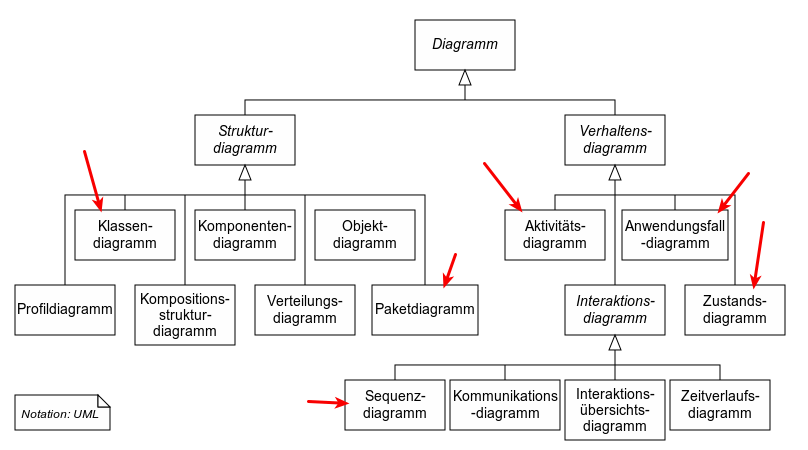
\includegraphics[scale=0.35]{./pics/tut1/uml_diagrams.png}
	\end{frame}	

	\begin{frame}[fragile]{UML-Klassendiagramm: Syntax}
	\begin{columns}
		\begin{column}{0.25\textwidth}
				\begin{tikzpicture}
				\centering
			\umlclass[name=classname]{Name der Klasse}{Attribute}{Methoden}
			\end{tikzpicture}
		\end{column}%
		\begin{column}{0.75\textwidth}
			\begin{itemize}
				\item Klassenname
				\begin{itemize}
					\item keine spezielle Syntax
					\item einfach Namen hinschreiben
				\end{itemize}
				\item Attribute
				\begin{itemize}
					\item \begin{verbatim}<modifier><name>:<type>\end{verbatim} 
				\end{itemize} 
				\item Methoden
				\begin{itemize}
					\item \begin{verbatim}<modifier><name>(<parameters>):<type>\end{verbatim}
					\item \verb|<parameters>|
					\begin{itemize}
						\item kann leer sein
						\item oder komma-getrennte Liste von \verb|<name>:<type>|
					\end{itemize}
					\item falls Rückgabe void, \verb|:<type>| weglassen
					
				\end{itemize} 
			\item statische Methoden und Attribute unterstreichen
			\end{itemize}
		\end{column}
	\end{columns}
\end{frame}

\begin{frame}{Modifier}
	\begin{itemize}
		\item UML
		\begin{itemize}
			\item -
			\begin{itemize}
				\item private
				\item von Instanzen derselben Klasse sichtbar (\textcolor{red}{aber von allen!})
			\end{itemize}
			\item \#
			\begin{itemize}
				\item protected (wie in Java)
				\item von Instanzen derselben Klasse, aller Unterklassen und Instanzen aus dem gleichen Paket sichtbar
			\end{itemize}
			\item +
			\begin{itemize}
				\item public (wie in Java)
				\item von Instanzen jeder Klasse sichtbar
			\end{itemize}
			\item falls nichts angegeben implizit public
		\end{itemize}
	\end{itemize}
\end{frame}

\begin{frame}{Beispiel}
\begin{figure}
	\centering
	\begin{tikzpicture}
		\umlclass[name=classname]{Hund}{- name: String\\
		- rasse: Rasse\\
		- gewicht: int}{
		+ wiegen(): int\\
		+ streicheln() \\
		+ streicheln(intensität: int, ausruf: String)\\
		+ füttern(ration: Nahrung)}
	\end{tikzpicture}
\end{figure}
\end{frame}
	
	\subsection{UML-Klassendiagramm (1)}
	\begin{frame}
		\frametitle{Vererbung}
		\begin{figure}
					\centering
			\begin{tikzpicture}
			\pgfsetlayers{connections,main}
				\umlclass[y=4,name=classname]
				{ParentClass}
				{+publicString: String \\
				-privateInt: int\\
				\#protectedDouble: double}
				{
				\umlstatic{+staticMethod()}\\
				+publicMethod(): String\\
				-privateMethod(): int\\
				\#protectedMethod(param: String): double
				}
			
				\umlemptyclass[y=0, name=classname]{ChildClass}
				
				\umlinherit{ChildClass}{ParentClass}
			\end{tikzpicture}
		\end{figure}
	\end{frame}
	
	\subsection{UML-Klassendiagramm (2)}
	\begin{frame}
		\frametitle{Interface}
				\begin{figure}
			\centering
			\begin{tikzpicture}
			\pgfsetlayers{connections,main}
			\umlclass[y=4,name=classname, type=interface]{NiceInterface}
			{}
			{
				+pleaseRealizeMe()
			}
			
			\umlclass[y=0, name=classname]{ImplementingClass}{}{+pleaseRealizeMe()}
			
			\umlimpl{ImplementingClass}{NiceInterface}
			\end{tikzpicture}
		\end{figure}
	\end{frame}
	
	\subsection{UML-Klassendiagramm (3)}
	\begin{frame}
		\frametitle{Abstrakte Klassen}
				\begin{figure}
			\centering
			\begin{tikzpicture}
			\pgfsetlayers{connections,main}
			\umlclass[y=3,name=classname,type=abstract]
			{AbstractClass}
			{}
			{
				+regularMethod(): String\\
				\umlvirt{+abstractMethod(): int}
			}
			
			\umlclass[y=0, name=classname]{ChildClass}{}{+abstractMethod(): int}
			
			\umlinherit{ChildClass}{AbstractClass}
			\end{tikzpicture}
		\end{figure}
	\end{frame}

	\begin{frame}
\frametitle{Abstrakte Klassen: Abgaben}
\begin{figure}
	\centering
	\begin{tikzpicture}
	\pgfsetlayers{connections,main}
	\umlclass[y=3,name=classname,tags={abstract}]
	{AbstractClass}
	{}
	{
		+regularMethod(): String\\
		+abstractMethod(): int \{abstract\}
	}
	
	\umlclass[y=0, name=classname]{ChildClass}{}{+abstractMethod(): int}
	
	\umlinherit{ChildClass}{AbstractClass}
	\end{tikzpicture}
\end{figure}
\begin{itemize}
	\item für Übungsblätter und Klausur
	\begin{itemize}
		\item kursiv nicht erkennbar, stattdessen \texttt{\{abstract\}} verwenden
		\item laut VL unter Klassenname, hinter Methode
	\end{itemize}
\end{itemize}
\end{frame}
	
	\subsection{UML-Klassendiagramm (4)}
	\begin{frame}
		\frametitle{Assoziationen}
		\begin{figure}
			\centering
			\begin{tikzpicture}
			\pgfsetlayers{connections,main}
			\umlclass[x=0,name=classname]
			{Firma}
			{angestellte: List$<$Person$>$}
			{}
			
			\umlclass[
			x=6, name=classname]{Person}{arbeitgeber: Firma}{}
			
			\end{tikzpicture}
		\end{figure}
	\pause
		\begin{alertblock}{Probleme}
			\begin{itemize}
				\item List$<$X$>$ ist Java-Syntax und schreibt Datenstruktur vor
				\item Beziehungen sollen direkt ersichtlich werden
				\item Faustregel: nur primitive Typen als Attribute hinschreiben
			\end{itemize}
		\end{alertblock}
				\begin{figure}
			\centering
			\begin{tikzpicture}
			\pgfsetlayers{connections,main}
			\umlclass[x=0,name=classname]
			{Firma}
			{}
			{}
			
			\umlclass[
			x=8, name=classname]{Person}{}{}
			
			\umlassoc[arg1=Arbeitgeber, arg2=Arbeitnehmer, mult1=0..1, mult2=*, pos1=0, pos2=1, align1=left, align2=right]{Firma}{Person}
			\end{tikzpicture}
		\end{figure}
	\end{frame}
	
	\subsection{UML-Klassendiagramm (5)}
	\begin{frame}
		\frametitle{Aggregation und Komposition}
		\begin{itemize}
			\item Aggregation = Teil-Ganzes-Beziehung
		\end{itemize}
			\begin{figure}
			\centering
			\begin{tikzpicture}
			\pgfsetlayers{connections,main}
			\umlclass[x=0,name=classname]
			{Auto}
			{}
			{}
			
			\umlclass[
			x=8, name=classname]{Rad}{}{}
			
			\umlaggreg[arg1=1, arg2=4, pos1=0, pos2=1, align1=left, align2=right, thick]{Auto}{Rad}
			\end{tikzpicture}
		\end{figure}
	\pause
		\begin{itemize}
			\item Komposition: Aggregation, aber Teil kann ohne Ganzes nicht existieren
			\begin{itemize}
				\item wenn ganzes gelöscht wird, dann auch Teile!
			\end{itemize}
		\end{itemize}
				\begin{figure}
		\centering
		\begin{tikzpicture}
		\pgfsetlayers{connections,main}
		\umlclass[x=0,name=classname]
		{Rechnung}
		{}
		{}
		
		\umlclass[
		x=8, name=classname]{Rechnungsposten}{}{}
		
		\umlcompo[arg1=1, arg2=1..*, pos1=0, pos2=1, align1=left, align2=right,thick]{Rechnung}{Rechnungsposten}
		\end{tikzpicture}
	\end{figure}
\end{frame}

	\subsection{UML-Warmup-Aufgabe}
	\begin{frame}
		\frametitle{Klassischer Aufgabentyp}
		\begin{exampleblock}{Text $\implies$ UML-Klassendiagramm}
			Jeder Student hat eine Matrikelnummer und einen Namen. Ein fauler Student ist ein Student, der schlafen kann. Er hat dazu ein Bett. Ein fleißiger Student hingegen, kann lernen und hat dazu einen Computer, der aus Bauteilen besteht.
		\end{exampleblock}
	\pause
	\textcolor{red}{UML-Diagramm?}
\end{frame}

	\subsection{UML-Warmup-Aufgabe2}
	\begin{frame}
	\frametitle{Klassischer Aufgabentyp}
	\begin{exampleblock}{Text $\implies$ UML-Klassendiagramm}
		Jeder \textcolor{red}{Student} hat eine Matrikelnummer und einen Namen. Ein fauler Student \textcolor{red}{ist ein} Student, der schlafen kann. Er \textcolor{red}{hat} dazu ein Bett. Ein fleißiger Student hingegen, kann lernen und \textcolor{red}{hat} dazu einen \textcolor{red}{Computer}, der aus \textcolor{red}{Bauteilen} \textcolor{red}{besteht}.
	\end{exampleblock}
	\textcolor{red}{Schlüsselwörter!}
\end{frame}
	
	\subsection{UML-Klausuraufgabe(1)}
	\begin{frame}
		\frametitle{Klausuraufgabe SS11}
		\textit{Modellieren Sie das Szenario möglichst vollständig als UML-Klassendiagramm. Geben Sie Methoden, Attribute, Multiplizitäten, Restriktionen, Assoziationsnamen, Aggregationen und Kompositionen sowie Rollen an.} 
		\begin{block}{Szenario}
			Ein Güterzug ist ein Zug, dessen Waggons ausschließlich Güterwagen sind. Die Waggons eines Personenzugs sind mindestens ein Reisezugwagen und höchstens ein Speisewagen. Jeder Zug hat eine oder zwei Lokomotiven. Reisezugwagen setzen sich aus bis zu einem Großraum sowie einem oder mehreren Abteilen zusammen. Jeder Reisezugwagen hat eine Klimaanlage, die ein- und ausgeschaltet werden kann. Jede Klimaanlage darf
			nur bis zu einer bestimmten maximalen Außentemperatur betrieben werden.
		\end{block}
	\end{frame}
	
	\subsection{UML-Klausuraufgabe(2)}
	\begin{frame}
		\frametitle{Musterlösung}
		\centering
		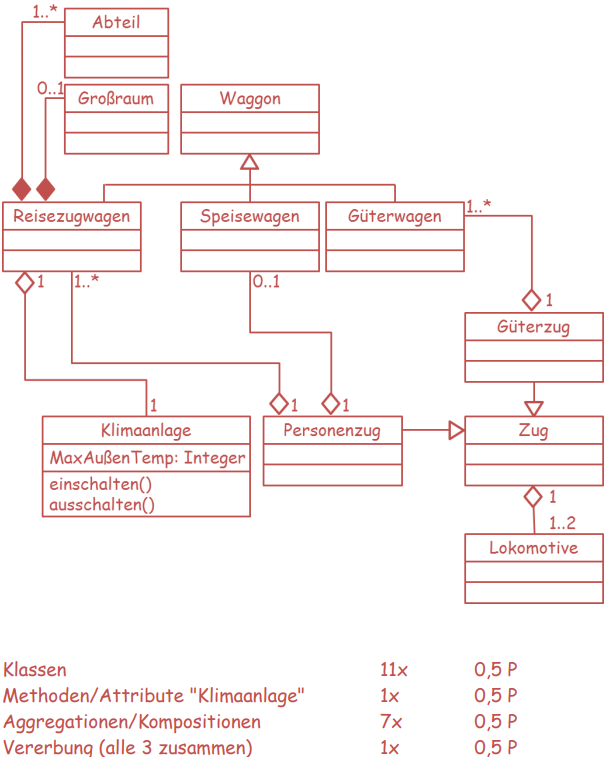
\includegraphics[scale=0.37]{./pics/tut1/solution.png}
	\end{frame}
		
		
\section{\LaTeX}
	\subsection{Basics}
	\begin{frame}
		\frametitle{\LaTeX - Basics}
		\begin{itemize}
			\item auf dem Blatt müsst ihr \LaTeX  ~ für die Dokumente benutzen
			\item wird euch an der Uni immer wieder begegnen, manchmal Pflicht
			\pause
			\item nicht WYSIWYG
			\begin{itemize}
				\item What You See Is What You Get
				\item Paradigma von Word etc.
			\end{itemize}
		\end{itemize}
		\begin{figure}
			\begin{subfigure}{0.5\textwidth}
				\centering
				\caption{\small What You See}
				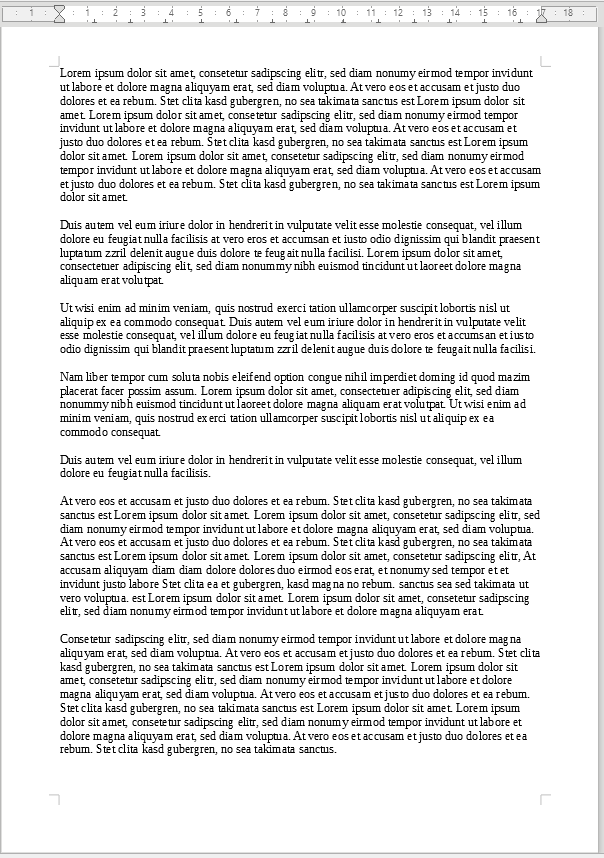
\includegraphics[scale=0.2]{pics/tut1/wysiwyg_raw.PNG}
			\end{subfigure}%
			\begin{subfigure}{0.5\textwidth}
				\centering
				\caption{\small What You Get}
				
\includegraphics[scale=0.2]{pics/tut1/wysiwyg.PNG}
			\end{subfigure}
		\end{figure}
	\end{frame}

\begin{frame}{\LaTeX - Basics}
	\begin{itemize}
		\item stattdessen WYSIWYAF bzw. WYSIWYM
		\begin{itemize}
			\item What You See Is What You Ask For / Mean
			\item Paradigma von \LaTeX $\approx$ HTML und CSS
		\end{itemize}
	\end{itemize}
	\begin{figure}
		\begin{subfigure}{0.55\textwidth}
			\centering
			\caption{\small What You See}
			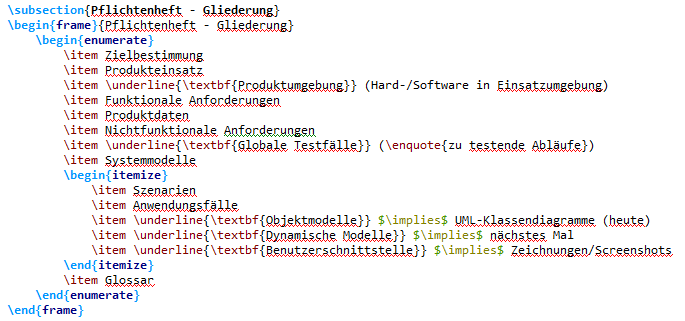
\includegraphics[scale=0.36]{pics/tut1/wysiwym_raw.PNG}
		\end{subfigure}%
		\begin{subfigure}{0.45\textwidth}
			\centering
			\caption{\small What You Mean}
			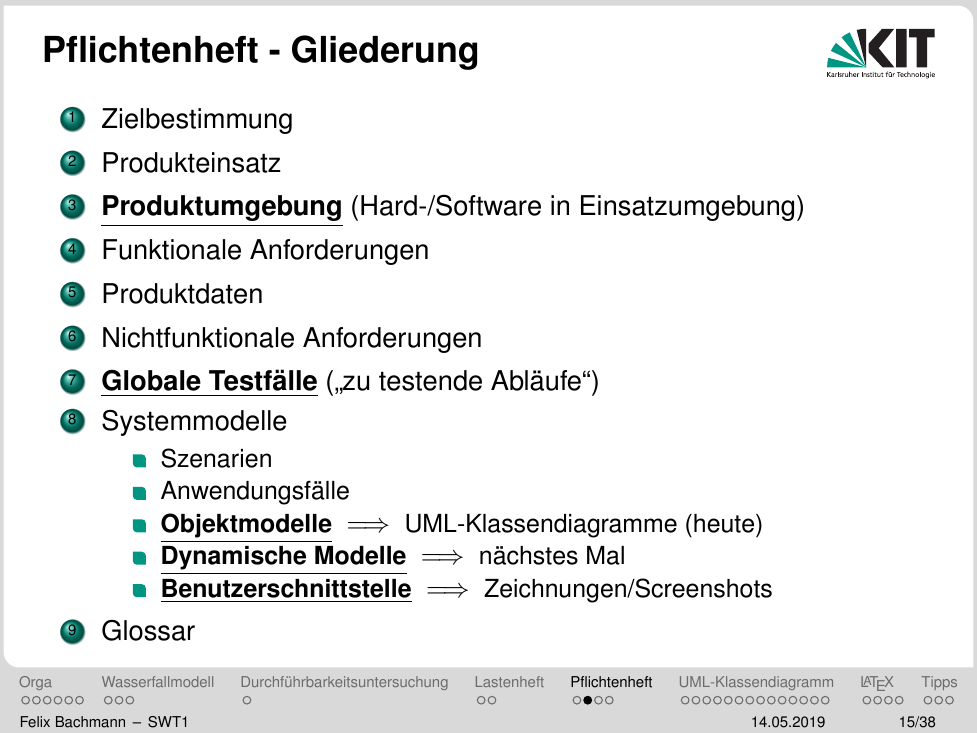
\includegraphics[scale=0.2]{pics/tut1/wysiwym.PNG}
		\end{subfigure}
	\end{figure}
\end{frame}

	\begin{frame}{\LaTeX}
	\begin{itemize}
		\item Vorteile
		\begin{itemize}
			\item gut versionierbar
			\begin{itemize}
				\item \enquote{Quellcode} ist normales Textdokument
				\item Word etc. verwenden oft XML-Formate mit Metadaten
			\end{itemize}
			\item leicht Formeln erstellbar
			\item nach Eingewöhnung recht intuitiv
			\item multifunktional (Bücher, Dokumente, Präsentationen, \dots)
			\item open source, kostet nix :)
			\item viele Erweiterungen, Pakete, \dots
		\end{itemize}
		\item Nachteile
		\begin{itemize}
			\item Einarbeitung notwendig :(
		\end{itemize} 
	\end{itemize}
				
\end{frame}
	
	\subsection{Installation}
	\begin{frame}
		\frametitle{\LaTeX - Installation}
		Installation einer Distribution notwendig, z.B.:
		\begin{itemize}
			\item  MiKTeX für Windows
			\item TeX Live für Linux, Mac, Windows
		\end{itemize}
		\pause
		Editoren machen das Schreiben von \LaTeX -Dokumenten angenehmer
		\begin{itemize}
			\item Texmaker
			\item TeXstudio (erweiterter Texmaker, mein Favorit)
			\item TeXclipse (Plugin für Eclipse)
			\item Plugins für Visual Studio Code
			\item \dots
		\end{itemize}
	\end{frame}
	
	\subsection{Beispiel}
	\begin{frame}
		\frametitle{\LaTeX - Dokumentaufbau}
		\begin{block}{Präambel: Pakete laden, Dokumenttyp festlegen}
			\texttt{$\backslash$documentclass\{Klasse\}} \newline
			\texttt{$\backslash$usepackage[option1,option2,\dots]\{Paket\}}
		\end{block}
		\begin{itemize}
			\item nützliche Klassen: book, beamer, scrartcl
			\item nützliches Paket z.B. csquotes (ermöglicht \texttt{$\backslash$enquote\{\dots\}})
		\end{itemize}
	\pause
		\begin{block}{Inhalt: Text setzen, Bilder, Graphiken, Formeln,\dots}
			\texttt{\% preamble \\ $\backslash$begin\{document\} \\ ~~~~content \\ $\backslash$end\{document\}}
		\end{block}
			\begin{itemize}
				\item Struktur: part, (chapter), section, subsection, subsubsection
				\item Auflistungen: $\backslash$begin\{itemize\} $\backslash$item Hello World! $\backslash$end\{itemize\}
				\item Bilder: $\backslash$includegraphics$[scale=0.8]$\{PfadZumBild\}
			\end{itemize}
	\end{frame}

\begin{frame}{}
	\huge \centering \textcolor{red}{\LaTeX-Beispiel!}
\end{frame}
		
\section{Tipps}
	\subsection{Tipps}
	\begin{frame}
		\frametitle{Tipps - 2. Übungsblatt}
		\begin{small}
			\begin{exampleblock}{Aufgabe 1 + 3: Lastenheft + Durchführbarkeitsuntersuchung}
				\begin{itemize}
					\item lasst euch was (sinnvolles) einfallen
					\begin{itemize}
						\item 6+3 Punkte für $<$ 5 Seiten sinnvollen Text! 
						\begin{itemize}
							\item besser wirds nicht
							\item aber: nicht zu allgemein werden, Bezug zu Szenario, Form
						\end{itemize}
					\end{itemize}
					\item Anwendungsfalldiagramm: Syntax beachten
					\item Durchführbarkeitsuntersuchung: Fragen beantworten, nicht stellen!
				\end{itemize}
			\end{exampleblock}
			\pause
			\begin{exampleblock}{Aufgabe 2: Klassendiagramme}
				\begin{itemize}
					\item Form, Syntax
					\item achtet auf Schlüsselwörter ("'ist ein"', "'enthält ein"', "'besteht aus"',\dots)
				\end{itemize}
			\end{exampleblock}
		\end{small}
	\end{frame}

	\begin{frame}
\frametitle{Tipps - 2. Übungsblatt}
	\begin{exampleblock}{Aufgabe 4 + 5: HDrize}
		\begin{itemize}
			\item HDR implementieren
			\begin{itemize}
				\item aus Belichtungsreihe
			\end{itemize}
			\item Zusammenhang der Klassen unklar? Vielleicht hilft Diagramm
		\end{itemize}
	\end{exampleblock}
\pause
	\begin{exampleblock}{Aufgabe 6: Schnittstellen für Filter}
		\begin{itemize}
			\item nur Schnittstellen definieren
			\item JavaDoc!
		\end{itemize}
	\end{exampleblock}
\end{frame}
	
	\subsection{Abgabe}
	\begin{frame}
		\frametitle{Denkt dran!}
		\begin{alertblock}{Abgabe}
			\begin{itemize}
				\item Deadline am 22.5 um 12:00
				\item Dokumente ausdrucken
				\item Klassendiagramme handschriftlich
				\item Deckblatt!
			\end{itemize}
		\end{alertblock}
	\end{frame}
		
	\begin{frame}
		\frametitle{Bis dann! (dann := 28.05.19)}
		\centering
		
\includegraphics[scale=0.86]{./comics/geek_and_poke_javadoc.jpg}
	\end{frame}

\end{document}
